\section{Ramanujanovi grafi}
Koncept ramanujanovih grafov ima enostavno definicijo, vendar njen pomen ni očiten brez predhodne motivacije s sorodnimi definicijami in izreki. Te nam razjasnijo povezavo med lastnimi vrednostmi grafa, ki se pojavijo v definiciji Ramanujanovih grafov, ter povezljivostjo grafa.
\subsection{Cheegerjeva konstanta}
Kot v uvodnem primeru nas zanima koliko povezav moremo odstraniti, da graf ni več povezan.

Naj bo \(G=(V,E)\) povezan graf in \(S\subseteq V\) podmnožica vozlišč z \(0<\abs{S} \leq \frac{\abs{V}}{2}\). Z \(\partial S\subseteq E\) označimo množico povezav od \(S\) do komplementa vozlišč, \(\overline{S}\). Če iz grafa odstranimo \(\partial S\), potem se graf postane nepovezan.

Najbolj problematična so ozka grla grafa. To je majhna množica povezav, ki ločuje dva dela grafa z veliko vozlišči. Da je graf dobro povezan torej želimo, da ni ozkih grl in da je za velik \(\abs{S}\) tudi velik \(\abs{\partial S} \), oziroma da \(\frac{\abs{S}}{\abs{\partial S}}\) ni nikoli majhen.

% reword T?
\begin{definicija}[Cheegerjeva konstanta]
    Za graf \(G = (V,E)\) in njegova vozlišča \(T = \left\{S\subseteq V \mid 0<\abs{S} \leq \frac{\abs{V}}{2}\right\}\) definiramo Cheegerjevo konstanto kot
    \begin{align*}
        c(G) = \min_{S\in T} \frac{\abs{\partial S}}{\abs{S}}
    \end{align*}
\end{definicija}
Večji kot je \(c(G)\), manj ozkih grl ima graf \(G\).

\begin{primer}[Cikli]
    \hspace{0em}
    \begin{center}
        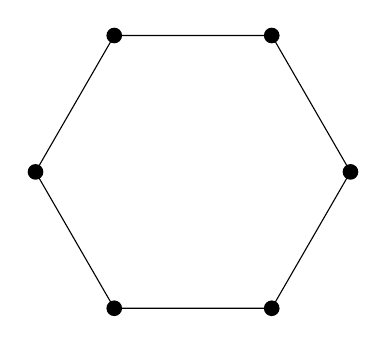
\begin{tikzpicture}
            % Defining the vertices of the cycle
            \foreach \x in {0,60,...,300} {
                    \node[circle, fill=black, inner sep=2pt] at (\x:2) {};
                }
            % Drawing the edges of the cycle
            \draw (0:2) -- (60:2) -- (120:2) -- (180:2) -- (240:2) -- (300:2) -- cycle;
        \end{tikzpicture}
    \end{center}

    Da minimiziramo \(\frac{\abs{\partial S}}{\abs{S}}\) lahko vzamemo sosednja vozlišča. Tako bo vedno \(\abs{\partial S} = 2\), \(S\) pa povečamo do polovice cikla, kot omejuje definicija. Za cikel \(C_{2n}\) torej vzamemo \(\abs{S} = n\), za \(C_{2n+1}\) pa prav tako \(\abs{S} = n\).
    \begin{align*}
        c(C_n) = \frac{2}{\lfloor \frac n2\rfloor}
    \end{align*}
    Večji kot je \(n\), manjša je Cheegerjeva konstanta in graf je slabše povezan, saj rabimo odstraniti le dve povezavi da ločimo veliko vozlišč od preostanka.
\end{primer}
\begin{primer}[Polni grafi]
    \hspace{0em}
    \begin{center}
        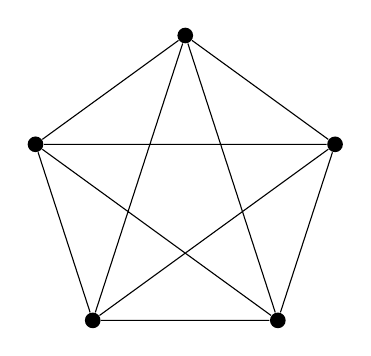
\begin{tikzpicture}
            \node[circle, fill=black, inner sep=2pt] (A) at (90:2) {};
            \node[circle, fill=black, inner sep=2pt] (B) at (162:2) {};
            \node[circle, fill=black, inner sep=2pt] (C) at (234:2) {};
            \node[circle, fill=black, inner sep=2pt] (D) at (306:2) {};
            \node[circle, fill=black, inner sep=2pt] (E) at (18:2) {};
            \draw (A) -- (B) -- (C) -- (D) -- (E) -- (A);
            \draw (A) -- (C) -- (E) -- (B) -- (D) -- (A);
        \end{tikzpicture}
    \end{center}
    Za graf \(K_n\) velja, da je \(\abs{\partial S} = \abs{S} \cdot (n - \abs{S})\). Torej je
    \begin{align*}
        c(K_n) = \min_{S} n-\abs{S}
    \end{align*}
    minimum je dosežen pri \(\abs{S} = \lfloor\frac n2\rfloor\) s poljubno izbiro vozlišč.
    \begin{align*}
        c(K_n) = \left\lceil \frac n2 \right\rceil
    \end{align*}
    Večji kot je \(n\), večja je Cheegerjeva konstanta in graf je bolje povezan.
\end{primer}
Oglejmo si še primer, kjer je zelo očitna povezava med ozkim grlom grafa in Cheegerjevo konstanto.
\begin{primer}[Ozko grlo]\hspace{0em}
    \begin{figure}
        \centering
        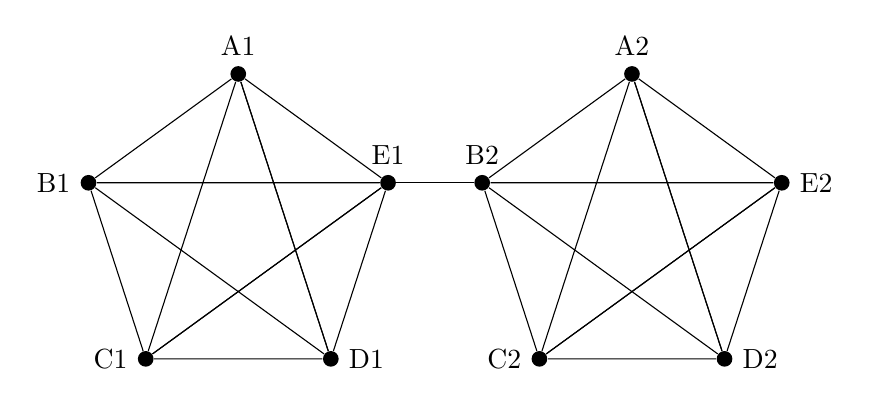
\begin{tikzpicture}
            % First K_5
            \begin{scope}[shift={(0,0)}]
                \node[circle, fill=black, inner sep=2pt, label=above:A1] (A1) at (90:2) {};
                \node[circle, fill=black, inner sep=2pt, label=left:B1] (B1) at (162:2) {};
                \node[circle, fill=black, inner sep=2pt, label=left:C1] (C1) at (234:2) {};
                \node[circle, fill=black, inner sep=2pt, label=right:D1] (D1) at (306:2) {};
                \node[circle, fill=black, inner sep=2pt, label=above:E1] (E1) at (18:2) {};
                \draw (A1) -- (B1) -- (C1) -- (D1) -- (E1) -- (A1);
                \draw (A1) -- (C1) -- (E1) -- (B1) -- (D1) -- (A1);
                \draw (A1) -- (D1);
                \draw (B1) -- (E1);
                \draw (C1) -- (E1);
            \end{scope}

            % Second K_5
            \begin{scope}[shift={(5,0)}]
                \node[circle, fill=black, inner sep=2pt, label=above:A2] (A2) at (90:2) {};
                \node[circle, fill=black, inner sep=2pt, label=above:B2] (B2) at (162:2) {};
                \node[circle, fill=black, inner sep=2pt, label=left:C2] (C2) at (234:2) {};
                \node[circle, fill=black, inner sep=2pt, label=right:D2] (D2) at (306:2) {};
                \node[circle, fill=black, inner sep=2pt, label=right:E2] (E2) at (18:2) {};
                \draw (A2) -- (B2) -- (C2) -- (D2) -- (E2) -- (A2);
                \draw (A2) -- (C2) -- (E2) -- (B2) -- (D2) -- (A2);
                \draw (A2) -- (D2);
                \draw (B2) -- (E2);
                \draw (C2) -- (E2);
            \end{scope}

            % Connecting edge between the two K_5 graphs
            \draw (E1) -- (B2);
        \end{tikzpicture}
        \caption{Povezana grafa \(K_5\)}
    \end{figure}
    Dvem polnim grafom \(K_n\) dodamo povezavo, da dobimo povezan graf \(G = (V,E)\). Če za \(S\) vzamemo enega izmed polnih grafov, je \(\abs{S} = n\) maksimalen in \(\abs{\partial S} = 1\) minimalen. Torej je Cheegerjeva konstanta
    \begin{align*}
        c(G) = \frac{1}{n}.
    \end{align*}
    Večji kot je \(n\), bolj izrazito je ozko grlo na grafu, kar vidimo tudi v manjši \(c(G)\).
\end{primer}
\subsection{Spektralna vrzel}
Graf lahko predstavimo tudi s sosednostno matriko. Vozlišča grafa \(G=(V,E)\) označimo od \(1\) do \(n=\abs{V}\) in naredimo \(n\times n\) matriko \(N(G)\), ki ima vrednost \(1\) na \((i,j)\)-tem mestu, če obstaja povezava med vozliščem \(i\) in \(j\) (oziroma \((i,j)\in E\)). Če povezave ni, je na tistem mestu vrednost \(0\).

Ker so grafi neusmerjeni je matrika simetrična. Po spektralnem izreku ima torej \(n\) realnih lastnih vrednosti \(\lambda_i\), ki jih uredimo po velikosti.
\begin{align*}
    \lambda_1 \geq \lambda_2 \geq \ldots \geq \lambda_n
\end{align*}

\begin{definicija}[Spektralna vrzel]
    Spektralna vrzel grafa \(G\) je razlika med dvema največjima lastnima vrednostima njegove sosednostne matrike.
    \begin{align*}
        s(G) = \lambda_1 - \lambda_2
    \end{align*}
\end{definicija}
\begin{primer}[Cikli]
    Graf \(C_n\) ima sosednostno matriko
    \begin{align*}
        N(C_n) = \begin{bmatrix}
                     0      & 1      & 0      & 0      & \cdots & 0      & 0      & 1      \\
                     1      & 0      & 1      & 0      & \cdots & 0      & 0      & 0      \\
                     0      & 1      & 0      & 1      & \cdots & 0      & 0      & 0      \\
                     \vdots & \vdots & \vdots & \vdots & \ddots & \vdots & \vdots & \vdots \\
                     0      & 0      & 0      & 0      & \cdots & 1      & 0      & 1
                 \end{bmatrix}.
    \end{align*}
    Matrika je cirkulantna, zato poznamo njene lastne vrednosti.
    \begin{align*}
        \lambda(N(C_n)) = \left\{ 2 \cos\left(\frac{2\pi k}{n}\right) \mid 0 \leq k \leq n-1\right\}
    \end{align*}
    % Add source?
    Od tod sledi, da je spektralna vrzel
    \begin{align*}
        s(C_n) = 2 - 2\cos\frac{2\pi}{n}.
    \end{align*}
    Opazimo da večji kot je graf, manjša je spektralna vrzel, prav tako kot je manjša Cheegerjeva konstanta.
\end{primer}
\begin{primer}[Polni grafi]
    Graf \(K_n\) ima sosednostno matriko
    \begin{align*}
        N(K_n) = \begin{bmatrix}
                     0      & 1      & 1      & \cdots & 1      \\
                     1      & 0      & 1      & \cdots & 1      \\
                     1      & 1      & 0      & \cdots & 1      \\
                     \vdots & \vdots & \vdots & \ddots & \vdots \\
                     1      & 1      & 1      & \cdots & 0
                 \end{bmatrix}.
    \end{align*}
    Lastne vrednosti matrike dobimo tako, da uganemo lastne vektorje.
    \begin{align*}
        v_1 = \begin{bmatrix}
                  1      \\
                  1      \\
                  \vdots \\
                  1
              \end{bmatrix} \\
        N(K_n) v_1 = (n-1) \cdot v_1
    \end{align*}
    Torej je ena lastna vrednost \(n-1\). Ostale lastne vektorje \(v_j\) za \(j>1\) dobimo kot
    \begin{align*}
        v_j = e_1 - e_j,
    \end{align*}
    kjer je \(e_j\) enotski vektor z \(1\) v \(j\)-ti komponenti. Ker je
    \begin{align*}
        N(K_n)v_j = -1 \cdot v_j,
    \end{align*}
    dobimo še \(n-1\) lastnih vrednosti \(-1\). Spektralna vrzel je torej
    \begin{align*}
        s(K_n) = (n-1) - (-1) = n.
    \end{align*}
    Opazimo da večji kot je graf, večja je vrzel (prav tako, kot je večja Cheegerjeva konstanta).
\end{primer}
\begin{primer}[Ozko grlo]
    Vzamemo primer dveh grafov \(K_n\), povezanih z eno povezavo. Matrika sosednosti je dimenzije \(2n \times 2n\) in ima na zgornji levi \(n\times n\) podmatriki vrednosti \(1\) povsod razen na diagonali, kjer so vrednosti \(0\). Enako je na spodnji desni \(n\times n\) podmatriki (tako dobimo dva grafa \(K_n\) kot podgrafa). Ostale vrednosti so \(0\), razen na elementu matrike \((1, n+1)\) in \((n+1, 1)\), kjer je vrednost \(1\) (ki predstavlja povezavo med grafoma \(K_n\)).

    Spektralne vrzeli izračunamo numerično in izrišemo na grafu.
    % compute/definicije_spectral_gap_bottleneck.py
    \begin{figure}[h!]
        \centering
        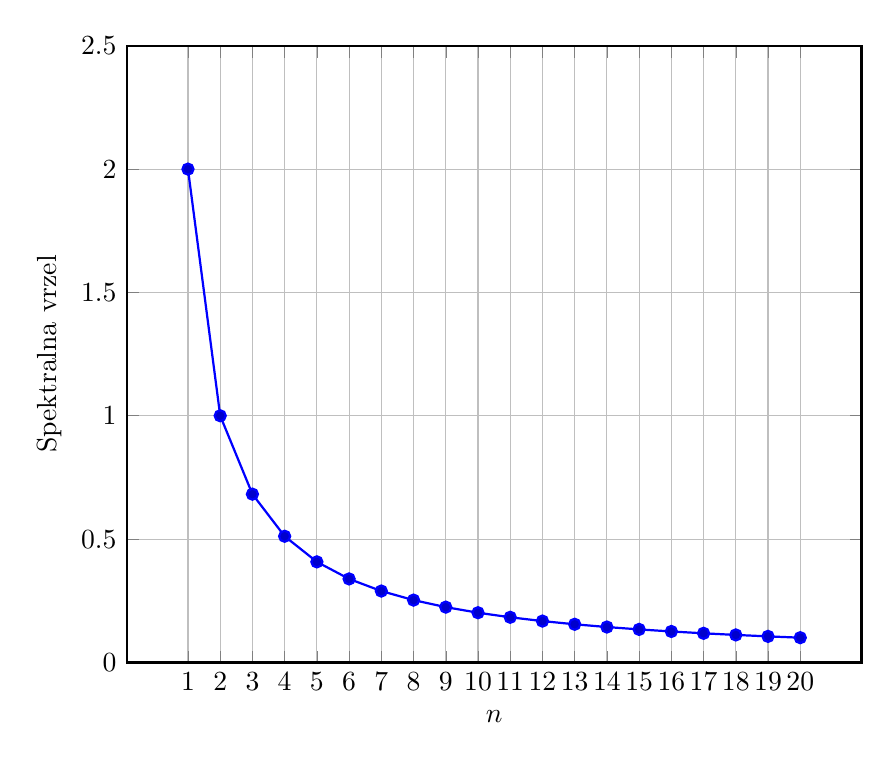
\begin{tikzpicture}
            \begin{axis}[
                    xlabel={$n$},
                    width=0.9\textwidth,
                    ylabel={Spektralna vrzel},
                    grid=major,
                    ymin=0, ymax=2.5,
                    xtick={1,2,...,20},
                    ytick={0,0.5,1,1.5,2,2.5},
                    thick
                ]
                \addplot coordinates {
                        (1, 2.0)
                        (2, 0.9999999999999988)
                        (3, 0.6821627548042195)
                        (4, 0.5114877902540731)
                        (5, 0.40764085275359996)
                        (6, 0.3384804373175667)
                        (7, 0.28929431396096117)
                        (8, 0.2525727509441946)
                        (9, 0.22412614005130305)
                        (10, 0.20144531545046007)
                        (11, 0.18293973049316747)
                        (12, 0.16755365441690628)
                        (13, 0.15455930002271145)
                        (14, 0.14343884532369877)
                        (15, 0.13381387867170424)
                        (16, 0.1254014671437087)
                        (17, 0.11798583829938813)
                        (18, 0.11139957046625426)
                        (19, 0.10551076707121965)
                        (20, 0.10021410708796452)
                    };
            \end{axis}
        \end{tikzpicture}
        \caption{Graf spektralnih vrzeli za \(n\) od 1 do 20}
    \end{figure}
    Opazimo, da večji kot je \(n\), manjša je spektralna vrzel, prav tako kot je manjša Cheegerjeva konstanta (in bolj kot je očitno ozko grlo).
\end{primer}

Računanje lastnih vrednosti regularnega grafa nam olajša tudi lastnost, da je njegova največja lastna vrednost enaka stopnji regularnosti.
\begin{izrek}[Največja vrednost \(d\)-regularnega grafa]
    Največja lastna vrednost \(d\)-regularnega grafa je \(d\).
\end{izrek}
\begin{dokaz}
    Lastni vektor \(d\)-regularnega grafa \(G\) za lastno vrednost \(d\) je vedno vektor samih enic, saj ima vsaka vrstica sosednostne matrike natanko \(n\) enic.

    Večje lastne vrednosti ne obstaja, saj so elementi sosednostne matrike samo \(0\) in \(1\). Če bi obstajala lastna vrednost \(\lambda > d\), potem si ogledamo največji element lastnega vektorja za to lastno vrednost, \(x\). Ker ima matrika natanko \(d\) enic v vsaki vrstici (in ostale vrednosti \(0\)), bi moralo obstajati \(d\) elementov vektorja, ki se skupaj sešteje v \(\lambda x\). Ker pa je vsak element manjši ali enak \(x\), imamo jih pa \(d\) lahko dosežemo kvečjemu \(d \times x\), torej večja lastna vrednost ne obstaja.
\end{dokaz}
Če je graf regularen torej, potrebujemo le izračunati njegovo drugo največjo lastno vrednost.
\subsection{Cheegerjeva neenakost}
Opazili smo, da se Cheegerjeva konstanta in spektralna vrzel obnašata podobno. Definiciji pa nista enakovredni - obstajajo na primer grafi, kjer lahko dodamo povezave ampak znižamo spektralno vrzel (medtem, ko bo Cheegerjeva konstanta ne more postati nižja).

\begin{primer}[Dodajanje povezave poviša vrzel]
    % compute/edges_increase_gap.py
    Kot primer vzamemo graf
    % change the labels to be as in the bottleneck example. Also make h! work
    \begin{figure}[h!]
        \centering
        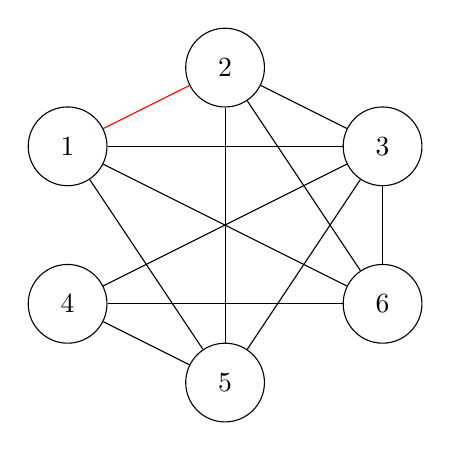
\begin{tikzpicture}[scale=1, every node/.style={circle, draw, minimum size=1cm}]
            % Nodes
            \node (1) at (0,2) {1};
            \node (2) at (2,3) {2};
            \node (3) at (4,2) {3};
            \node (4) at (0,0) {4};
            \node (5) at (2,-1) {5};
            \node (6) at (4,0) {6};

            % Edges based on the adjacency matrix
            \path[draw=red] (1) edge (2);
            \path (1) edge (3);
            \path (1) edge (5);
            \path (1) edge (6);

            \path (2) edge (3);
            \path (2) edge (5);
            \path (2) edge (6);

            \path (3) edge (4);
            \path (3) edge (5);
            \path (3) edge (6);

            \path (4) edge (5);
            \path (4) edge (6);
        \end{tikzpicture}
    \end{figure}
    s sosednostno matriko
    \begin{align*}
        \begin{bmatrix}
            0          & \mathbf{1} & 1 & 0 & 1 & 1 \\
            \mathbf{1} & 0          & 1 & 0 & 1 & 1 \\
            1          & 1          & 0 & 1 & 1 & 1 \\
            0          & 0          & 1 & 0 & 1 & 1 \\
            1          & 1          & 1 & 1 & 0 & 0 \\
            1          & 1          & 1 & 1 & 0 & 0 \\
        \end{bmatrix}.
    \end{align*}
    Spektralna vrzel grafa je približno \(3.706\), če pa odstranimo povezavo med vozliščema \(1\) in \(2\) dobimo spektralno vrzel približno \(3.766\). Tako smo graf naredili slabše povezanega, spektralno vrzel pa vseeno povišali. Cheegerjeva konstanta pa je v obeh primerih enaka \(2\) (kjer za \(S\) lahko vzamemo vozlišča \(1\), \(2\) in \(5\)).
\end{primer}

Kljub temu pa lahko povezavo med konceptoma Cheegerjeve neenakosti in spektralne vrzeli vseeno formaliziramo.
\begin{izrek}[Cheegerjeva neenakost]
    Za \(d\)-regularen graf \(G\) velja 
    \begin{align*}
        \frac{1}{2}s(G) \leq c(G) \leq \sqrt{2ds(G)}
    \end{align*}
    oziroma
    \begin{align*}
        2c(G) \geq s(G) \geq \frac{c(G)^2}{2d}
    \end{align*}    
\end{izrek}
Za dokaz izreka potrebujemo naslednjo lemo.
\begin{lema}\label{cheegerLema}
    Za poljubna \(a, b, c, d > 0\) velja
    \begin{align*}
        \frac{a+b}{c+d} \geq \min\left(\frac{a}{c}, \frac{b}{d}\right).
    \end{align*}
\end{lema}
\begin{dokaz}
    \begin{align*}
        a+b &= c\cdot\frac{a}{c} + d\cdot \frac{a}{d}\\
        a+b &\geq (c+d) \min\left(\frac{a}{c}, \frac{b}{d}\right)\\
        \frac{a+b}{c+d} &\geq \min\left(\frac{a}{c}, \frac{b}{d}\right)
    \end{align*}
\end{dokaz}
\begin{dokaz}[Dokaz Cheegerjeve neenakosti]
    Dokažimo najprej \(2c(G) \geq s(G)\). Naj bo \(S\subset V(G)\) tak, da zadosti minimumu iz definicije Cheegerjeve konstante, torej \(0<\abs{S} \leq \frac12\abs{V(G)}\) in 
    \begin{align*}
        c(G) = \frac{\abs{\partial S}}{\abs{S }}.
    \end{align*}
    Spektralno vrzel poiščemo prek Rayleighovega kvocienta. Če je \(A\) sosednostna matrika grafa je Rayleighov kvocient
    \begin{align*}
        R(A, v) = \frac{v^\top Av}{v^\top v}.
    \end{align*}
    Vemo že, da je vektor samih enic lastni vektor sosednostne matrike za največjo lastno vrednost \(d\). Če torej želimo drugo največjo lastno vrednost, lahko poiščemo maksimum Rayleighovega kvocienta po vseh vektorjih, ki so pravokotni na vektor samih enic. Da pokažemo želeno neenakost izberemo specifičen vektor \(v\) in izračunamo njegov Rayleighov kvocient. Druga največja lastna vrednost bo večja ali enaka od izračunanega kvocienta, spektralna vrzel pa zato manjša.

    Izberemo vektor \(v\) tako, da ima elemente enake \(\frac{1}{\abs{S}}\) na indeksih, ki pripadajo elementom iz \(S\) ter ostale elemente (tiste, ki pripadajo indeksom za \(\overline S\)) enake \(-\frac{1}{\abs{\overline S}}\). Ta vektor je pravokoten na vektor samih enic.
    Sedaj izračunamo Rayleighov kvocient.
    \begin{align*}
        Av = \left(\sum_{j=1}^{\abs{V(G)}} v_j \cdot A_{i,j}\right)_{i=1}^{\abs{V(G)}}\\
        v^\top Av = \sum_{i=1}^{\abs{V(G)}} \sum_{j=1}^{\abs{V(G)}} v_i v_j A_{i,j} = \sum_{i\sim j} v_i v_j\\
    \end{align*}
    \begin{align*}
        R(A, v) &= \frac{\sum_{i\sim j} v_i v_j}{\sum_{i=1}^{\abs{V(G)}}v_i^2}\\
        &= \frac{\sum_{i\sim j} v_i^2 + v_j^2 - \left(v_i - v_j\right)^2}{2 \sum_{i=1}^{\abs{V(G)}}v_i^2}\\
        &= \frac{\sum_{i\sim j} v_i^2}{\sum_{i=1}^{\abs{V(G)}}v_i^2} - \frac{\sum_{i\sim j}\left(v_i - v_j\right)^2}{2 \sum_{i=1}^{\abs{V(G)}}v_i^2}\\
        &= \frac{d\cdot \sum_{i=1}^{\abs{V(G)}}v_i^2}{\sum_{i=1}^{\abs{V(G)}}v_i^2} -  \frac{2\cdot \sum_{i\in S \land j \in \overline S}\left(v_i - v_j\right)^2}{2 \sum_{i=1}^{\abs{V(G)}}v_i^2}\\
        &= d - \frac{\abs{\partial S} \cdot \left(\frac{1}{\abs{S}} + \frac{1}{\abs{\overline S}}\right)^2}{\abs{S} \frac{1}{\abs{S}^2} + \abs{\overline S} \frac{1}{\abs{\overline S}^2}}\\
        &= d - \abs{\partial S}\left(\frac{1}{\abs{S}} + \frac{1}{\abs{\overline S}}\right) \\ 
        &= d - \frac{\abs{\partial S}}{\abs{S}}\frac{\left(\abs{S} + \abs{\overline S}\right)}{\abs{\overline S}}\\
        &= d- c(G) \frac{V(G)}{\abs{\overline S}}\\
        &\geq d - 2c(G)
    \end{align*}
    Torej velja
    \begin{align*}
        \lambda_2 \geq R(A,v) \geq d-2c(G)\\
        2c(G) \geq d-\lambda_2 = s(G)
    \end{align*}

    % file:///home/tadej/library/math/magistrska/cheeger_chung.pdf
    Sedaj dokažemo še drugo neenakost, \(s(G) \geq \frac{c(G)^2}{2d}\). Tu bomo preko Fiedlerjevega algoritma s pomočjo lastnega vektorja za drugo največjo lastno vrednost konstruirali particijo grafa.

    Naj bo \(v\) lastni vektor za drugo največjo lastno vrednost, \(\lambda_2\). Brez škode za splošnost preuredimo vozlišča grafa tako, da je \(v_i \geq v_j\) za \(i < j\). Definiramo \(S_i = \{v_1, \ldots, v_i\}\) in 
    \begin{align*}
        \alpha(G) = \min_{1\leq i \leq V(G)/2} \frac{\abs{\partial S_i}}{\abs{S_i}}.
    \end{align*}
    Očitno je \(h(G) \leq \alpha(G)\).

    Vzamemo \(r=\floor{\frac{V(G)}{2}}\) in definiramo
    \begin{align*}
        v^+_i = \begin{cases}
            v_i - v_r & v_i \geq v_r \\
            0 & v_i < v_r
        \end{cases}\\
        v^-_i = \begin{cases}
            v_r - v_i & v_i \leq v_r \\
            0 & v_i > v_r
        \end{cases}.
    \end{align*}
    Predpostavimo, da velja \(R(A, v^+) \geq R(A, v^-)\), sicer lastni vektor \(v\) pomnožimo z \(-1\). Izbrali smo \(r\) tako, da bosta vedno oba vektorja (\(v^+\) in \(v^-\)) imela kvečjemu \(r\) pozitivnih elementov, kar se ohrani, če zamenjamo predznake v vektorju \(v\), kot zahteva predpostavka. Vozlišča, ki pripadajo pozitivnim elementom \(v^+\) bomo uporabili pri vpeljavi \(\alpha(G)\), ki pa zahteva podgraf velikosti največ \(r\). Predpostavko lahko zapišemo tudi drugače:
    \begin{align}\label{eq:cheegerPredpostavka}
        \frac{\sum_{i\sim j}(v^+_i - v^+_j)^2}{2\sum_{i=1}^{\abs{V(G)}} (v^+_i)^2} \leq \frac{\sum_{i\sim j} (v^-_i - v^-_j)^2}{2\sum_{i=1}^{\abs{V(G)}} (v^-_i)^2} 
    \end{align}

    Podobno kot v prvem delu dokaza preko Rayleighovega kvocienta izrazimo spektralno luknjo.
    \begin{align*}
        s(G) &= d-\lambda_2 \\ 
        &= \frac{\sum_{i\sim j}(v_i - v_j)^2}{2\sum_{i=1}^{\abs{V(G)}} v_i^2}
    \end{align*}
    
    Ker je \(v\) pravokoten na največji lastni vektor, vektor samih enic, velja \(\sum_i v_i = 0\). Tako lahko povečamo imenovalec kvocienta:
    \begin{align*}
        \sum_{i=1}^{\abs{V(G)}} v_i^2 = \min_{c\in \R} \sum_{i=1}^{\abs{V(G)}} (v_i - c)^2 \leq \sum_{i=1}^{\abs{V(G)}} (v_i - v_r)^2\\
        \frac{\sum_{i\sim j}(v_i - v_j)^2}{2\sum_{i=1}^{\abs{V(G)}} v_i^2} \geq \frac{\sum_{i\sim j}(v_i - v_j)^2}{2\sum_{i=1}^{\abs{V(G)}} (v_i-v_r)^2}
    \end{align*}
    Imenovalec lahko prepišemo z uporabo \(v^+\) in \(v^-\)
    \begin{align*}
        \frac{\sum_{i\sim j}(v_i - v_j)^2}{2\sum_{i=1}^{\abs{V(G)}} v_i^2} \geq \frac{\sum_{i\sim j}(v_i - v_j)^2}{2\sum_{i=1}^{\abs{V(G)}} (v_i-v_r)^2} = \frac{\sum_{i\sim j}(v_i - v_j)^2}{2\sum_{i=1}^{\abs{V(G)}} (v^+_i)^2 + 2\sum_{i=1}^{\abs{V(G)}} (v^-_i)^2}.
    \end{align*}
    
    Sedaj pomanjšamo števec \(\sum_{i\sim j}(v_i - v_j)^2\). Če sta \(v_i\) in \(v_j\) oba večja od \(v_r\), potem velja
    \begin{align*}
        (v_i - v_j)^2 = (v^+_i - v^+_j)^2 + (v^-_i - v^-_j)^2.
    \end{align*}
    Enako velja, če sta oba manjša od \(v_r\). V primeru ko je \(v_j \leq v_r \leq v_i\), pa vidimo slednje:
    \begin{align*}
        0 \geq (v_r - v_i)(v_r - v_j)\\
        0 \geq v_r^2 - v_r v_i - v_r v_j + v_i v_j \\
        -2 v_i v_j \geq 2 v_r^2 - 2 v_r v_i - 2 v_r v_j \\
        v_i^2 - 2v_i v_j + v_j^2 \geq (v_r^2 - 2v_r v_i + v_i^2) + (v_r^2 - 2v_r v_j + v_j^2) \\ 
        (v_i - v_j)^2 \geq (v_i - v_r -0)^2 + (0 + v_j - v_r)^2 \\
        (v_i - v_j)^2 \geq  (v^+_i - v^+_j)^2 + (v^-_i - v^-_j)^2
    \end{align*}
    Enako velja v primeru \(v_i \leq v_r \leq v_j\), torej je
    \begin{align*}
        s(G) &\geq \frac{\sum_{i\sim j}(v_i - v_j)^2}{2\sum_{i=1}^{\abs{V(G)}} (v^+_i)^2 + 2\sum_{i=1}^{\abs{V(G)}} (v^-_i)^2}\\
        &\geq \frac{\sum_{i\sim j}(v^+_i - v^+_j)^2 + (v^-_i - v^-_j)^2}{2\sum_{i=1}^{\abs{V(G)}} (v^+_i)^2 + 2\sum_{i=1}^{\abs{V(G)}} (v^-_i)^2}
    \end{align*}
    
    Zgornjo neenakost lahko, s pomočjo predpostavke \eqref{eq:cheegerPredpostavka} in leme \ref{cheegerLema} spremenimo v

    \begin{align*}
        s(G) \geq  \frac{\sum_{i\sim j}(v^+_i - v^+_j)^2}{2\sum_{i=1}^{\abs{V(G)}} (v^+_i)^2}.
    \end{align*}
    Od tod sledi
    \begin{align*}
        s(G) &\geq  \frac{\sum_{i\sim j}(v^+_i - v^+_j)^2}{2\sum_{i=1}^{\abs{V(G)}} (v^+_i)^2} \frac{\sum_{i\sim j}(v^+_i + v^+_j)^2}{\sum_{i\sim j}(v^+_i + v^+_j)^2}\\
        &= \frac{\sum_{i\sim j}(v^+_i - v^+_j)^2}{2\sum_{i=1}^{\abs{V(G)}} (v^+_i)^2} \frac{\sum_{i\sim j}(v^+_i + v^+_j)^2}{\sum_{i\sim j}(v^+_i)^2 + (v^+_j)^2 + 2v^+_i v^+_j}\\
        &= \frac{\sum_{i\sim j}(v^+_i - v^+_j)^2}{2\sum_{i=1}^{\abs{V(G)}} (v^+_i)^2} \frac{\sum_{i\sim j}(v^+_i + v^+_j)^2}{2d\sum_{i=1}^{\abs{V(G)}} (v^+_i)^2 + 2\sum_{i\sim j}v^+_i v^+_j}
    \end{align*}
    Uporabimo Cauchy-Schwarzovo neenakost ločeno na števcu in na delu imenovalca.
    \begin{align*}
        s(G) &\geq  \frac{\left(\sum_{i\sim j}(v^+_i - v^+_j)(v^+_i + v^+_j)\right)^2}{2\sum_{i=1}^{\abs{V(G)}} (v^+_i)^2\left(2d\sum_{i=1}^{\abs{V(G)}} (v^+_i)^2 + 2\sqrt{\sum_{i\sim j}(v^+_i)^2 \sum_{i\sim j} (v^+_j)^2}\right)}\\
        &= \frac{\left(\sum_{i\sim j}\abs{(v^+_i)^2 - (v^+_j)^2} \right)^2}{2\sum_{i=1}^{\abs{V(G)}} (v^+_i)^2 \left(2d\sum_{i=1}^{\abs{V(G)}} (v^+_i)^2 + 2d \sum_{i=1}^{\abs{V(G)}}(v^+_i)^2 \right)}\\
        &= \frac{\left(\sum_{i\sim j}\abs{(v^+_i)^2 - (v^+_j)^2} \right)^2}{8d\left(\sum_{i=1}^{\abs{V(G)}} (v^+_i)^2\right)^2}\\
        &= \frac{\left(2\sum_{i\sim j \land i< j}(v^+_i)^2 - (v^+_j)^2 \right)^2}{8d\left(\sum_{i=1}^{\abs{V(G)}} (v^+_i)^2\right)^2} \\
        &= \frac{\left(\sum_{i\sim j \land i< j}(v^+_i)^2 - (v^+_j)^2 \right)^2}{2d\left(\sum_{i=1}^{\abs{V(G)}} (v^+_i)^2\right)^2}
    \end{align*}
    Vsak sumand \((v^+_i)^2 - (v^+_j)^2\) lahko teleskopsko razpišemo kot
    \begin{align*}
        (v^+_i)^2 &- (v^+_{i+1})^2\\
        + (v^+_{i+1})^2 &- (v^+_{i+2})^2\\
        + &\cdots\\
        + (v^+_{j-1})^2 &- (v^+_{j})^2,
    \end{align*}
    da dobimo
    \begin{align*}
        s(G) &\geq \frac{\left(\sum_{i=1}^{\abs{V(G)}}\abs{\partial S_i}\left((v^+_i)^2 - (v^+_{i+1})^2\right) \right)^2}{2d\left(\sum_{i=1}^{\abs{V(G)}} (v^+_i)^2\right)^2}
        &=\frac{\left(\sum_{i=1}^{r}\abs{\partial S_i}\left((v^+_i)^2 - (v^+_{i+1})^2\right) \right)^2}{2d\left(\sum_{i=1}^{r} (v^+_i)^2\right)^2}
    \end{align*}
    Po definiciji za vsak \(i\leq r\) velja \(\abs{\partial S_i} \geq \abs{S_i} \alpha(G)\).
    \begin{align*}
        s(G) &\geq \frac{\left(\sum_{i=1}^{r} \abs{S_i} \alpha(G)\left((v^+_i)^2 - (v^+_{i+1})^2\right) \right)^2}{2d\left(\sum_{i=1}^{r} (v^+_i)^2\right)^2}\\
        &= \frac{\alpha(G)^2}{2d} \frac{\left(\sum_{i=1}^{r} \abs{S_i}\left((v^+_i)^2 - (v^+_{i+1})^2\right) \right)^2}{\left(\sum_{i=1}^{r} (v^+_i)^2\right)^2}\\
        &= \frac{\alpha(G)^2}{2d} \frac{\left(\sum_{i=1}^{r} i\cdot (v^+_i)^2 - \sum_{i=1}^{r} (i-1) \cdot (v^+_{i})^2 \right)^2}{\left(\sum_{i=1}^{r} (v^+_i)^2\right)^2}\\
        &= \frac{\alpha(G)^2}{2d} \frac{\left(\sum_{i=1}^{r} i\cdot (v^+_i)^2 - \sum_{i=1}^{r} (i-1) \cdot (v^+_{i})^2 \right)^2}{\left(\sum_{i=1}^{r} (v^+_i)^2\right)^2}\\
        &= \frac{\alpha(G)^2}{2d} \frac{\left(\sum_{i=1}^{r} \cdot (v^+_i)^2 \right)^2}{\left(\sum_{i=1}^{r} (v^+_i)^2\right)^2}\\
        &= \frac{\alpha(G)^2}{2d}\\
    \end{align*}
    Tako dobimo
    \begin{align*}
        s(G) \geq \frac{\alpha(G)^2}{2d} \geq \frac{h(G)^2}{2d}
    \end{align*}



\end{dokaz}
\subsection{Alon-Boppanov izrek}
\subsection{Ramanujanovi grafi}